\documentclass[tikz]{standalone}

% tikz picture of a flash drum with heat exchanger and pressure
% reducing valve.

\usepackage[scaled]{helvet}
\renewcommand\familydefault{\sfdefault} 
\usepackage[T1]{fontenc}

\usepackage{sansmath}
\begin{document}

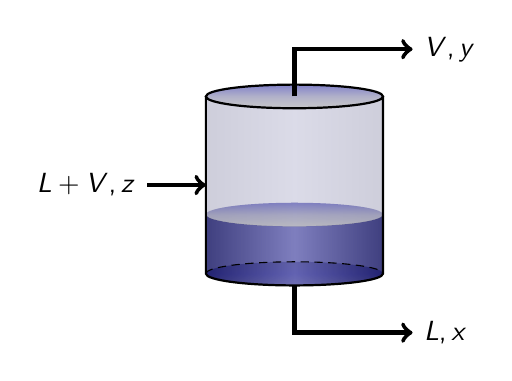
\begin{tikzpicture}[scale=0.75]
\begin{sansmath}
%\draw[step=1cm,gray,very thin] (-3,-1) grid (3,5);
%\node (blank) at (5,1) {};
% bottom disk
\fill[
    top color=blue!50!black,
    bottom color=blue!10,
    middle color=blue,
    shading=axis,
    opacity=0.25] (0,0) circle (1.5cm and 0.2cm);
    
% volume vapor
\fill[left color=blue!50!black,
    right color=blue!50!black,
    middle color=blue!50,
    shading=axis,
    opacity=0.1] (1.5,1)
    -- (1.5,3) arc (360:180:1.5cm and 0.2cm)
    -- (-1.5,1) arc (180:360:1.5cm and 0.2cm);
    
% top vapor disk
\fill[top color=blue!90!,
    bottom color=blue!2,
    middle color=blue!30,
    shading=axis,opacity=0.3] (0,3) circle (1.5cm and 0.2cm);

% volume liquid
\fill[left color=blue!50!black,
    right color=blue!50!black,
    middle color=blue!50,
    shading=axis,
    opacity=0.5] (1.5,0)
    -- (1.5,1) arc (360:180:1.5cm and 0.2cm)
    -- (-1.5,0) arc (180:360:1.5cm and 0.2cm);

% top liquid disk
\fill[top color=blue!90!,
    bottom color=blue!2,
    middle color=blue!30,
    shading=axis,opacity=0.25] (0,1) circle (1.5cm and 0.2cm);

% cylinder outline
\draw[thick] (-1.5,3) -- (-1.5,0) arc (180:360:1.5cm and 0.2cm)
    -- (1.5,3) ++ (-1.5,0) circle (1.5cm and 0.2cm);

\draw[densely dashed] (-1.5,0) arc (180:0:1.5cm and 0.2cm);

\draw[<-,ultra thick] (-1.5,1.5) -- ++(-1,0) node[left] {$L+V, z$};
\draw[->,ultra thick] (0,-0.2) -- ++(0,-0.8) 
    -- ++(2,0) node[right] {$L,x$};
\draw[->,ultra thick] (0,3) -- ++(0,0.8) 
    -- ++(2,0) node[right] {$V, y$};

\end{sansmath}
\end{tikzpicture}

\end{document}